% !TEX root = ../../report.tex

\section{Mathematische Verfahren}

\subsection{Verzerrung von Bildern}

\subsection{Blending}
Blending ist ein Verfahren welches es ermöglicht überlappende Teilbereiche von zwei Objekten zu definieren.
Hierbei spielt der Alpha-Kanal eine große Rolle, dieser besagt wie durchsichtig ein Objekt ist und somit die Dominanz beim mischen von Farben. Es gibt verschiedene Ausprägungen des Blendings, im einfachsten Fall - so wie auch in unserem Projekt, kommt das additive Alpha-Blending zum Einsatz. Besitzt der Alpha Wert einen hohen Wert (nahe 1) so ist das Objekt sehr dominant und kaum bis garnicht durchsichtig. Ist der Alpha Wert hingegen niedrig (nahe 0) so ist das Objekt durchsichtig vergleiche hierzug Abbildung \ref{fig:AlphaBlending}.
\begin{figure}[h!]
	\centering
	\vspace*{30px}
	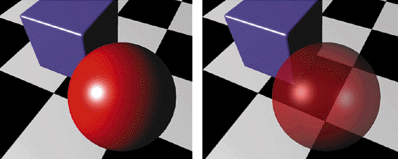
\includegraphics[width=320px]{graphics/blending.png}	
	\caption{Additives Alpha-Blending\protect\footnotemark}
	\label{fig:AlphaBlending}
\end{figure}
\footnotetext{Quelle: \url{http://common.ziffdavisinternet.com/encyclopedia_images/_ALPHACH.GIF}}

\subsection{Billboarding}
Um unsere Vorgabe der Echtzeitfähigkeit zu erfüllen benötigt es ein paar Tricks, die es erlauben die Komplexität unseres Renderers zu minimieren, gleichzeitig jedoch darf der Zuschauer diese Manipulation nicht bemerken.
Eine beliebte Technik hierfür ist das Billboarding. Die Idee des Billboardings basiert darauf, komplexe geometrische 3D-Objekte auf ein zweidimensionales Rechteck das sogenannte Billboard runterzubrechen. 
Bei dem Billboard handelt es sich meist um ein vorher berechnetes Bild von dem ursprünglich darzustellenden 3D-Objekts.
Anschließend wird dieses Billboard zur Kamera ausgerichtet. Durch den zusätzlichen Einsatz von Blending überlappen diese 2D Objekte Objekte dann und erzeugen somit einen 3D-Effekt. Dem Zuschauer fällt es somit sehr schwer zu erkennen, das es sich bei dem gezeigten Objekt um eine zweidimensionale Kopie des 3D-Objektes handelt.
Diese Technik wird hauptsächlich dazu verwendet die benötigten Rechenoperationen für Objekte welche in der Ferne liegen zu minimieren. 
Kommt die Kamera dem tatsächlichen Objekten sehr nahe, wird meist mittels einer Interpolation zwischen dem Billboard und dem tatsächlichen 3D-Objekt umgeschaltet.
\end{Spacing}
\newpage
\clearpage
%% End Of Doc